\documentclass{article}
\usepackage[utf8]{inputenc}
\usepackage{graphicx}
\usepackage{amsmath}
\usepackage{parskip}
\graphicspath{ {images/} }

\begin{document}
\begin{center}
\huge\bf Elliptic Curve Cryptography 
\newline
\newline
\end{center}






\begin{center}
   
    \setlength{\fboxrule}{.5mm}\setlength{\fboxsep}{1.2mm}
	\newlength{\boxlength}\setlength{\boxlength}{\textwidth}
	\addtolength{\boxlength}{-4mm}
	\begin{center}\framebox{\parbox{\boxlength}{\bf
             	Professors: Manish Gupta\\[10pt]
				Group Members and their Contribution
				\newline
				\begin{enumerate}
				    \item Soham Viradiya(202101472)\\
				    Contribution:
				    \newline 
				    
				    \item Jay Sabva(202101224)\\
				    Contribution:
				    \newline
				    
				    \item Shrut Kalathiya(202101479)\\
				    Contribution:
				    \newline
				    
				    \item Vasu Golakiya(202101487)\\
				    Contribution:
				    \newline
				    \item Vandit Bhalani(202101478)\\
				    Contribution: 
				    \newline
				    \item Dev Changela(202101069)\\
				    Contribution:
				    \newline
				    \item Swet Lakhani(202101218)\\
				    Contribution:
				    \newline
				    
				\end{enumerate}
	}}
	\end{center} 
	\vspace{5mm}
\end{center}






\newpage
\section{Introduction and History of Cryptography}
The History of cryptography can be split into two eras:the classical era and the modern era. The turning point between the two occurred in 1977, when both the RSA algorithm and the Diffie-Hellman key exchange algorithms were introduced.These new algorithms were revolutionary because they represented the first viable cryptographic schemes where security was based on the theory of numbers; it was the first to enable secure communication between two parties without a shared secret.Cryptography went from being about securely transporting secret codebooks around the world to being able to have provably secure communication between any two parties without worrying about someone listening in on the key exchange.

Modern cryptography is founded on the idea that the key that you use to encrypt your data can be made public while the key that is used to to decrypt your data can be kept private. As such, these systems are known as public key cryptographic systems. The first, and still most widely used of these systems, is known as RSA — named after the initials of the three men who first publicly described the algorithm: Ron Rivest, Adi Shamir and Leonard Adleman.

What you need for a public key cryptographic system to work is a set of algorithms that is easy to process in one direction, but difficult to undo. In the case of RSA, the easy algorithm multiplies two prime numbers. If multiplication is the easy algorithm, its difficult pair algorithm is factoring the product of the multiplication into its two component primes. Algorithms that have this characteristic — easy in one direction, hard the other — are known as Trap door Functions. Finding a good Trapdoor Function is critical to making a secure public key cryptographic system. Simplistically: the bigger the spread between the difficulty of going one direction in a Trapdoor Function and going the other, the more secure a cryptographic system based on it will be.



\begin{figure}[hb]
  \centering
  \begin{minipage}[hb]{0.3\textwidth}
    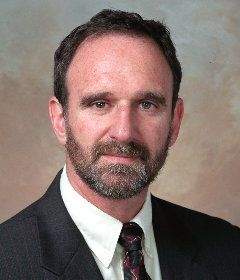
\includegraphics[width=\textwidth]{Martin-Hellman.jpg}
    \caption{Martin Hellman}
  \end{minipage}
  \hfill
  \begin{minipage}[hb]{0.3\textwidth}
    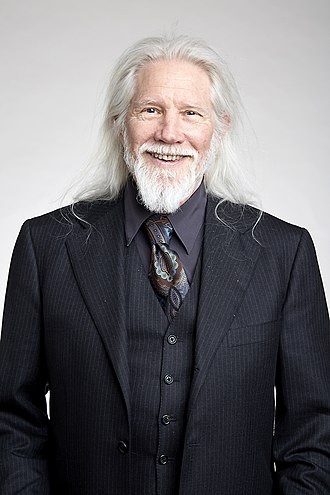
\includegraphics[width=\textwidth]{Diffle.jpg}
    \caption{Whitefield Diffle}
  \end{minipage}
\end{figure}


\end{document}
